\chapter{Modellierung und Entwurf}
\label{cha:Modellierung und Entwurf}

In diesem Kapitel werden die funktionalen Anforderungen aus dem Abschnitt \ref{sec:anforderungsdefinition} spezifiziert. Modelle für die einzelnen funktionalen Anforderungen sollen entwickelt werden. Die Modelle veranschaulichen das geforderte funktionale Verhalten der Software. Voraussetzung für die Entwicklung der Modelle ist die Konkretisierung der funktionalen Anforderungen. Diese Konkretisierung beinhaltet die Festlegung der Bestandteile die für eine Implementierung der funktionalen Anforderung benötigt werden. Ziel des Kapitels ist es, die wichtigsten Bestandteile einer funktionalen Anwendung herauszubilden, dieses Bestandteile zu definieren und zu veranschaulichen. 

\section{Tic Tac Toe}
\label{sec:Tic Tac Toe}

Das klassische Tic Tac Toe ist ein Spiel, welches mit genau zwei Spielern gespielt wird. Jeder dieser Spieler setzt abwechselnd entweder ein Kreuz oder einen Kreis. Während eines gesamten Spiels darf ein Spieler nur Kreuze setzen und der andere Spieler nur Kreise. Wir können uns die Kreuze und Kreise als Spielfiguren vorstellen, die sobald sie auf das Spielfeld gesetzt wurden, nicht mehr verändert oder verschoben werden können. Das Spielfeld ist eine drei mal drei große Matrix, also können maximal neun Spielfiguren in diese Matrix gesetzt werden. Im ersten Spielzug stehen dem Spieler neun mögliche Positionen zur Verfügung. Die Anzahl der möglichen Positionen reduziert sich jede Runde um eins. Folglich ist die maximale Länge einer Spielzugsequenz, bei einem drei mal drei Spielfeld, neun. Maximal deshalb, weil das Spiel auch vor der neunten Runde bereits entschieden sein kann. \\

\subsection{Spielregeln}
\label{subsec:Spielregeln}

Ziel des Spiels ist es vier Kreuze oder vier Kreise in einer bestimmten Position anzuordnen. Es wird davon ausgegangen, dass zwei Spieler Alice und Bob existieren und gegeneinander Tic Tac Toe spielen. Alice setzt ausschließlich Kreuze und Bob ausschließlich Kreise. Wir gewähren Alice in unseren Beispielen immer den ersten Zug. Es existieren drei unterschiedliche Anordnungen von Spielfiguren, die das Spiel beenden und einen Sieg herbeiführen. Gewinnt ein Spieler mit einer Siegesanordnung seiner Spielfiguren, dann verliert der andere Spieler dadurch automatisch in gleicher Höhe (Nullsummenspiel). \\

\begin{figure}[!htbp]
  \centering
  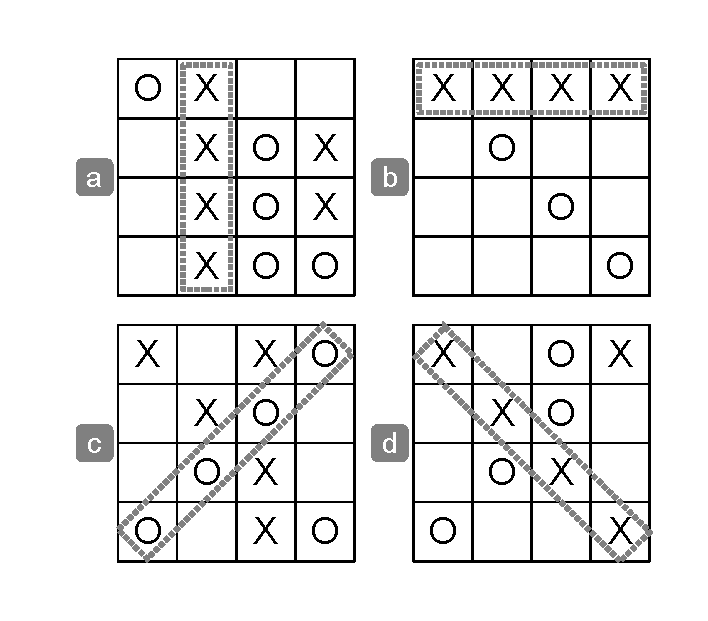
\includegraphics[scale = 1]{inhalt/abbildungen/siegesbedingungen_tictactoe.pdf}
  \caption{Veranschaulichung der vertikalen (a), horizontalen (b) und diagonalen (c, d) Siegesbedingung.}
  \label{fig:siegesbedingungen_tictactoe}
\end{figure}

In Abbildung \ref{fig:siegesbedingungen_tictactoe} a, gewinnt Alice knapp gegen Bob mit einer ununterbrochenen vertikalen Anordnung ihrer Spielfiguren. Bob hätte fast eine diagonale Reihe aus Kreisen verbunden, diese wurde jedoch von Alice mit einer Spielfigur geblockt. Zudem hätte Bob auch fast eine vertikale Spalte ohne Unterbrechungen vervollständigt. Eine horizontale Siegesanordnung entsteht, wenn vier Spielfiguren eines Spielers in einer horizontalen Zeile angeordnet sind. Alice gewinnt das zweite Spiel gegen Bob durch eine horizontale Siegesanordnung (siehe Abbildung \ref{fig:siegesbedingungen_tictactoe} b). In jeder Spalte des Spielfeldes ist genau eine vertikale und in jeder Zeile des Spielfeldes ist genau eine horizontale Siegesanordnung möglich. Die dritte und letzte Anordnungsvariante der Spielfiguren, welche zu einem Sieg eines Spielers führt, ist die diagonale Verbindung von vier Spielfiguren eines Spielers. In Abbildung  \ref{fig:siegesbedingungen_tictactoe} c, gewinnt Bob mit einer diagonalen Anordnung von vier Spielfiguren ohne Unterbrechung einer gegnerischen Spielfigur. Alice gewinnt ebenfalls eine Party, durch einen diagonale Siegesanordnung (Abbildung \ref{fig:siegesbedingungen_tictactoe} d). Eine Party wird, in diesem Kontext, als ein abgeschlossenes Spiel, mit anschließendem Ergebnis, verstanden. \\

Bei einem vier mal vier Spielfeld existieren vier vertikale, vier horizontale und zwei diagonale Anordnungen der Spielfiguren, welche einen Sieg herbeiführen würden. Insgesamt zehn verschiedene Siegesanordnungen für beide Spieler. Was passiert jedoch, wenn keine der zehn möglichen Siegesanordnungen auftritt, dann gewinnt beziehungsweise verliert keiner der beiden Spieler und es entsteht ein Unentschieden. Sind die beiden Kontrahenten gleich gut, erfahren oder verwenden die selben Strategien, dann tritt ein Unentschieden möglicherweise öfter oder andauernd ein.

\subsection{Suchbaum}

\begin{figure}[!htbp]
  \centering
  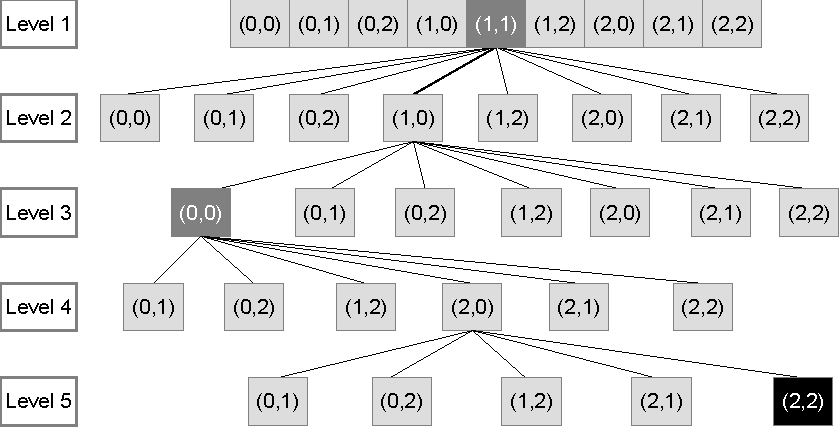
\includegraphics[scale = 1]{inhalt/abbildungen/suchbaum_drei_mal_drei_tictactoe.pdf}
  \caption{TicTacToe Spielbaum, eines drei mal drei Spielfeldes, der in Level fünf terminiert.}
  \label{fig:drei_mal_drei_tictactoe_spielbaum}
\end{figure}

Ein Suchbaum für ein drei mal drei Spielfeld, hat maximal eine Tiefe (Level) von neun. Der Verzweigungsfaktor im ersten Level ist äquivalent zur maximalen Tiefe des Suchbaums. Für jedes weitere Level reduziert sich der Verzweigungsfaktor um eins. In Level eins ist der Verzweigungsfaktor gleich neun, in Level fünf ist er gleich fünf und in Level neun ist er gleich  eins. Der Verzweigungsfaktor reduziert sich deshalb in jedem Spielzug, weil in jedem Spielzug eine Position mit einer Spielfigur besetzt wird und eine bereits besetzte Position darf nicht erneut besetzt werden. Der Sieg mit der kürzesten Spielzugsequenz ist nach fünf Spielzügen, für den beginnenden Spieler, zu erreichen. Bob der erst als zweites seinen Spielzug ausführen darf, kann erst ab einer Spielzugsequenz der Länge sechs gewinnen. Abbildung \ref{fig:drei_mal_drei_tictactoe_spielbaum} zeigt einen schwarz markierten terminierenden Endzustand (2,2) des Spielbaums in Level fünf. Alice erreicht diesen Endzustand, weil sie ihren Spielstein in Zeile zwei und Spalte zwei setzt. Die terminierenden Endzustände des Spielbaumes werden allgemein als Blattknoten bezeichnet. Ein Blattknoten charakterisiert, dass es keine weiteren Verzweigungen oder Knoten unterhalb dieses Blattknotens geben darf. \todo{Ist jeder Blattknoten ein Terminierender Endzustand?} Es gibt zwei Möglichkeiten für das erreichen eines Blattknotens(Bedingung der Terminierung):

\begin{enumerate}
\item Eine Siegesanordnung ist entstanden.
\item Alle möglichen Positionen des Spielfeldes sind besetzt und es wurde keine Siegesanordnung erreicht.
\end{enumerate}

In Level fünf bis Level neun können terminierende Endzustände auftreten, das heißt Alice kann in Level fünf, Level sieben und in Level neun eine Siegesformation erreichen. Bob hingegen kann in Level sechs und Level acht eine Siegesanordnung erhalten. Theoretisch fehlt Bob, dem Spieler der als zweites beginnt, ein Zug gegenüber dem zu erst beginnenden Spieler. Tritt ein terminierender Endzustand von Level fünf bis Level acht auf, dann wurde dieser Endzustand immer durch das erreichen einer Siegesanordnung hervorgerufen, sprich durch die 1. Bedingung der Terminierung. Ein Blattknoten in Level neun kann durch die 1. und 2. Bedingung der Terminierung entstehen, das heißt entweder ist das Spielfeld voll besetzt und es wurde keine Siegesanordnung gefunden oder das Spielfeld ist voll besetzt und es wurde eine Siegesanforderung gefunden. Folglich besteht Level neun ausschließlich aus Blattknoten. \\

5 * 8 * (3 * 3)
40 terminierende Endzustände

Wie viele verschiedene Zustände kann ein drei mal drei Tic Tac Toe Spielfeld haben?
Eine beliebige regelkonforme Anordnung von Spielsteinen auf dem Tic Tac Toe Spielfeld bezeichnen wir als einen Zustand $s_1$. Eine Menge die alle möglichen Zustände s enthält bezeichnen wir als die Menge S. Somit gilt $s_1, s_2 ... s_x \in S$. Der gesamte Spielbaum eines drei mal drei Tic Tac Toe Spielfeldes (Spielbaum ähnelt Abbildung \ref{fig:drei_mal_drei_tictactoe_spielbaum}) hat
 
\begin{equation}
\prod_{i=1}^{9} 9 - (i - 1) = 9 \times 8 \times 7 \times 6 \times 5 \times 4 \times 3 \times 2 \times 1 = 362880
\end{equation}

Blattkonten. In dieser Rechnung sind keine Positionsredundanzen und terminierende Endzustände berücksichtigt.
 

\begin{equation}
\prod_{i=0}^{5 - 1} 9 - i = 9 \times 8 \times 7 \times 6 \times 5 = 15120
\end{equation}

Um die Anzahl der möglichen Spielzüge zu erhöhen und um die mittlere unfaire Position in einem drei mal drei Spielfeld zu entfernen, wird das Spielfeld des klassischen Tic Tac Toe auf eine vier mal vier Matrix erweitert.

\subsection{Lernen mit Strategieverbesserung}
Die nachfolgend aufgestellte Strategie ist keine optimale Strategie, das heißt es ist nicht möglich mit dieser Strategie immer zu gewinnen oder mindestens ein Unentschieden zu erreichen. Das Ziel des Lernverfahrens ist es, diese nicht optimale Strategie in eine optimale Strategie oder zumindest eine annähernd optimale Strategie zu transformieren. Eine optimale Strategie würde gegen unaufmerksame oder unerfahrene Gegner verhältnismäßig oft Gewinnen und nicht gegen diese Verlieren, Unentschieden können trotzdem vorkommen. Ist der Gegner ein perfekter TicTacToe Algorithmus oder ein TicTacToe Großmeister, dann sollte die optimale Strategie überwiegend Unentschieden hervorbringen. Eine optimale Strategie sollte in 100 Spielen gegen einen Großmeister oder eine andere optimale Strategie (dieselbe optimale Strategie oder möglicherweise eine andere) 100 Unentschieden erringen. Siege sind theoretisch höherwertiger als Unentschieden, aber innerhalb der TicTacToe Spielwelt sind diese gegen einen Großmeister oder einen perfekten Algorithmus äußerst unwahrscheinlich. \\

Unser Lernalgorithmus oder im Kontext des verstärkenden Lernens unser Agent, erhält eine Belohnung von +1 wenn er eine Party (eine komplette Spielzugsequenz bis ein Spielergebnis feststeht) TicTacToe gewinnt. Verliert er eine Party, dann wird er bestraft mit dem numerischen Wert -1. Bei einem Unentschieden wird der Agent ebenfalls belohnt, aber die Belohnung ist nicht so hoch wie bei einem Sieg, denn wir wollen das Verhalten des Lernverfahrens so trainieren, dass es eher einen Sieg erlangen wird als ein Unentschieden, aber auf jeden Fall eine Niederlage vermeidet. Der Agent soll immer versuchen diesen nummerischen Wert zu maximieren, darum wird er eine Niederlage vermeiden. Der Agenten könnte auch so trainiert werden, dass er immer absichtlich verlieren würde, dafür müsste jeder, vom Agenten ausgeführte, Spielzug (egal welcher Spielzug) eine hohe negative nummerische Bestrafung hervorbringen. Das Ziel des Agenten wäre dann, schnellstmöglich ein Ende des Spiels zu provozieren und weil verlieren sicherer und kürzer ist als gewinnen oder ein Unentschieden, würde der Agent lernen absichtlich zu verlieren. Interessant wäre das Spielergebnis, wenn zwei Agenten gegeneinander antreten würden, die immer schnellstmöglich verlieren wollen, dann entstünden theoretisch ausschließlich Unentschieden.


\myparagraph{Kombination von überwachtem und verstärkenden Lernen}
Dem Lernverfahren eine Strategie vorzugeben, welche für jeden Zustand festlegt welche Aktion ausgeführt werden soll, ähnelt stark dem überwachten Lernen. Bei einem überwachten Lernverfahren würde der Agent eine Liste von Zuständen und Aktionen als Eingabeparameter bekommen, in dieser Liste sind den Zuständen Aktion zugeordnet. Der Agent lernt die Liste von Zustand-Aktions-Paaren und dadurch lernt er, bei welcher Spielfiguren Anordnung (Zustand), welche Position mit seiner Spielfigur belegt werden sollte (Aktion). Die Zustände wären in diesem Trainingsset Eigenschaften (Features) und die Aktionen wären Zielvariablen (Target Values). In der Theorie wird überwachtes Lernen mit verstärkendem Lernen kombiniert, um ein schnell konvergierendes Lernverfahren zu erhalten. Die Konvergenz bezieht sich auf die Strategie, welche das Lernverfahren optimieren soll. Der Agent versucht diese nicht optimale Strategie schrittweise in eine optimale Strategie umzuwandeln und wenn ihm dies gelingt, dann hat die verbesserte nicht optimale Strategie eine Konvergenz mit der optimalen Strategie erreicht, dass bedeutet die Ausgangsstrategie wurde zu einer optimale Strategie weiterentwickelt. \\

Warum eigentlich kein reines überwachtes oder verstärkendes Verfahren? Eine optimale Strategie nur durch überwachtes Lernen zu erstellen, würde ein Trainingsset voraussetzen, indem jeder Zustand der Spielwelt erfasst ist und jeder dieser Zustände müsste genau eine optimale Aktion abbilden. Bei komplexeren Probleme kann das sehr hohe Kosten verursachen oder es ist überhaupt nicht möglich, denn für viele Zustände ist die optimale Aktion nicht bekannt. Das vier mal vier TicTacToe ist noch ein recht simpler Vertreter der Strategiespiele und soll dazu dienen, die Anwendung und Modellierung der Lernverfahren und der Strategien zu veranschaulichen. Ob ein Strategiespiel im Kontext der Lernverfahren simpler oder komplexer ist ,hängt von seinen Zustands- und Aktionsdimensionen ab. Die Größe das Spielfelds, die Anzahl verschiedener Aktionen pro Spielsituation und die durchschnittliche Anzahl der Spielzüge, entscheiden über die Komplexität des Strategiespiels. Wenn das überwachte Lernen einer optimalen Strategie aufgrund größerer Dimensionen nicht möglich ist, können wir dann nicht ein verstärkendes Lernverfahren implementieren? \\

Unterabschnitt \ref{subsec:Lernen ohne Strategie} behandelt die Thematik des reinen verstärkenden Lernens. Daher werden die Vor- und Nachteile des reinen verstärkenden Lernens jetzt nicht weiter analysiert. Wir konzentrieren uns in diesem Abschnitt darauf, welche Strategien entwickelt, wie diese Strategien praktisch angewendet und wie die angewendeten Strategien optimiert werden können. Bei der Entwicklung der Strategie muss besonders darauf geachtet werden, worauf der Agent aufmerksam gemacht werden soll. Unter Umständen ist es besonders Wahrscheinlich zu gewinnen, wenn eine besondere Spielstellung erreicht wurde oder  einzelne Spielfelder erleichtern einen Sieg und sollten daher eher besetzt werden als andere möglicherweise unwichtigerer Spielfelder. Die Ausgangsstrategie ist also ein wichtiger Faktor für die Konvergenz-Geschwindigkeit.

\myparagraph{Das Spielfeld}

\begin{figure}[!htbp]
  \centering
  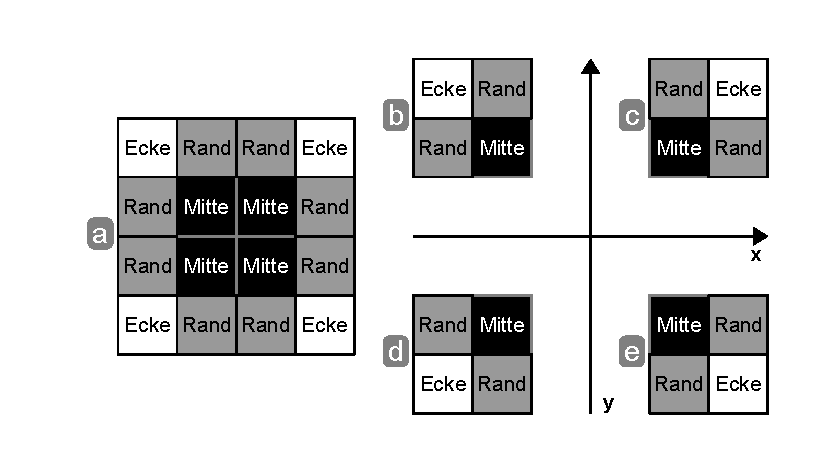
\includegraphics[scale = 1]{inhalt/abbildungen/symmetrie_tictactoe_spielfeld.pdf}
  \caption{Symmetrie Eigenschaften des vier mal vier Tic Tac Toe Spielfelds.}
  \label{fig:symmetrie_tictactoe_spielfeld}
\end{figure}

Um eine Strategie zu entwickeln werden wir uns zuerst das Spielfeld ansehen und dieses analysieren. Das vier mal vier TicTacToe Spielfeld hat 16 Spielfelder, vier Eckfeldern, vier Mittelfeldern und acht Randfeldern (siehe Abbildung \ref{fig:symmetrie_tictactoe_spielfeld} a). Ziehen wir eine horizontale und eine vertikale Achse durch das Spielfeld, dann sind bestimmte Symmetrieeigenschaften zu erkennen, Abbildung \ref{fig:symmetrie_tictactoe_spielfeld} zeigt b und c, sowie d und e sind symmetrisch zur y-Achse, b und d, sowie c und e sind symmetrisch zur x-Achse und b und e, sowie d und c sind symmetrisch, wenn man sie an der x-Achse und der y-Achse spiegelt. Diese Symmetrieeigenschaften sind wichtig für die Reduktion der Strategien, das heißt wenn eine Strategie auf b angewendet werden kann, dann auch auf c, d und e.

\myparagraph{Kontrolliere die Mitte}

Um über bestimmte Spielfelder reden zu können, müssen wir eine konkrete Identifikation der einzelnen Spielfelder vornehmen. In Abbildung \ref{fig:tictactoe_spielfeld_indizes} wird daher jedem der Spielfelder ein Index zugewiesen.

\begin{figure}[!htbp]
  \centering
  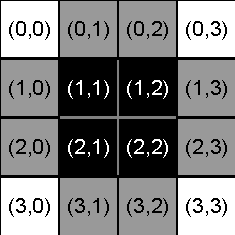
\includegraphics[scale = 1]{inhalt/abbildungen/tictactoe_spielfeld_indizes.pdf}
  \caption{Die Indizes der einzelnen Spielfelder.}
  \label{fig:tictactoe_spielfeld_indizes}
\end{figure}

Die Eröffnungsstrategie konzentriert sich auf die Kontrolle der Mittelfelder. Hat der Agent beziehungsweise das Lernverfahren das Recht auf den ersten Zug befindet er sich immer in Zustand $s_0$. In diesem Zustand sind alle Spielfelder leer und der Agent kann durch Zufall eines der vier mittleren Felder wählen. Der Agent trifft diese Entscheidung zufällig, weil zu diesem Zeitpunkt und in diesem Zustand alle vier Mittelfelder die gleiche positive numerische Belohnung erbringen (siehe Abbildung \ref{fig:kontrolliere_die_mitte} 1). Die Rand- und Eckfelder haben keine numerische Belohnung, aber auch keine numerische Bestrafung für den Agenten, so wird sichergestellt, dass das Lernverfahren sich für ein mittleres Spielfeld entscheidet. Nachdem der gegnerische Spieler seine Spielfigur gesetzt hat, soll der Agent die zweite Spielfigur ebenfalls auf ein mittleres Feld setzen, jedoch eher auf ein mittleres Spielfeld, welches sich in einer Reihe ohne eine gegnerische Spielfigur befindet. \\

\begin{figure}[!htbp]
  \centering
  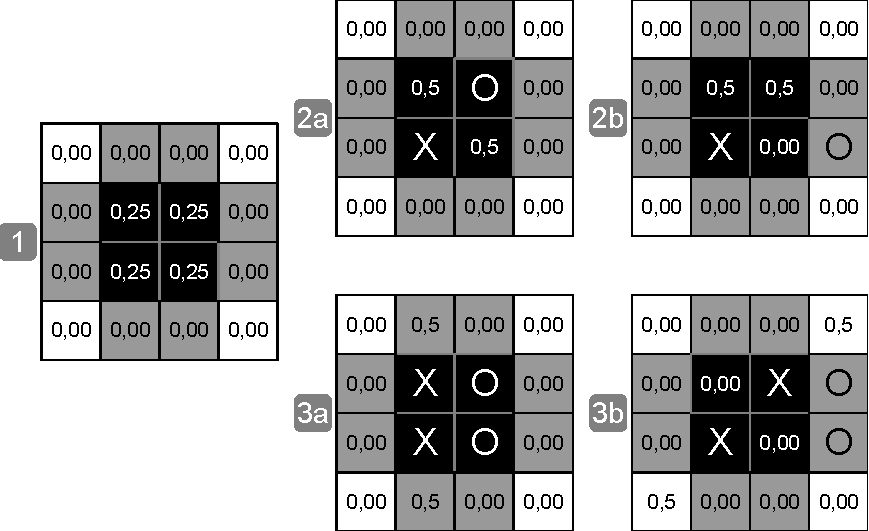
\includegraphics[scale = 0.8]{inhalt/abbildungen/kontrolliere_die_mitte.pdf}
  \caption{Strategie um die Mitte zu kontrollieren.}
  \label{fig:kontrolliere_die_mitte}
\end{figure}

Von jetzt an betrachten wir die beiden Kontrahenten Alice (Spielfiguren X) und Bob (Spielfiguren O) als zwei Instanzen des selben Lernverfahrens, dass heißt der Agent spielt gegen einen anderen Agenten mit exakt dem selben Verhalten.
In Abbildung \ref{fig:kontrolliere_die_mitte} (2a) setzt Alice ihre Spielfigur auf das Feld (2,1) und Bob auf (1,2). Die Strategie der Mittelfeld Kontrolle offenbart unserer Agentin Alice zwei Aktionsmöglichkeiten mit positiver Belohnung. Setzt Agentin Alice ihre Spielfigur auf die Mittelfelder (1,1) oder (2,2), dann erhält sie einen numerische Belohnung von +0,5. Alice entscheidet durch Zufall welches der beiden Felder mit der gleichgroßen größtmöglichen Belohnung sie auswählt. Alice entscheidet sich durch Zufall für das Spielfeld (1,1) und Bob, der ebenfalls der Strategie der Mittelfeld Kontrolle folgt, entscheidet sich für das letzte nicht besetzte Mittelfeld (Abbildung \ref{fig:kontrolliere_die_mitte} 3a).\\

Sollte Agent Bob eine andere gelernte Strategie verfolgen und zum Beispiel ein Randfeld besetzen, dann werden Agentin Alice andere Aktionen von ihrer Strategie Vorgeschlagen. In einem alternativen Spielverlauf (Abbildung \ref{fig:kontrolliere_die_mitte} 2b) setzt Agent Bob seine Spielfigur nicht auf das Spielfeld (1,2), sondern auf das Spielfeld (2,3). Die Strategie der Kontrolle der Mittelfelder bevorzugt Mittelfelder, die in einer leeren vertikalen, horizontalen oder diagonalen Reihe sind, bezogen auf die bereits gesetzte Spielfigur. Das Mittelfeld (2,2) wird uninteressant für die Strategie von Alice, weil eine mögliche horizontale Reihe aus vier gleichen Spielsteinen bereits nicht mehr möglich ist. Dahingegen schlägt die Strategie die Mittelfelder (1,1) und (1,2) mit einer numerischen Belohnung von +0,5 vor. Setzt Alice ihre Spielfigur auf das Mittelfeld (1,1), dann ist eine vertikale Verbindung von vier gleichen Spielfiguren möglich und setzt Alice ihre Spielfigur auf das Mittelfeld (1,2), dann ist eine diagonale Verbindung von vier gleichen Spielfiguren möglich. \\

Agentin Alice entschiedet durch Zufall ihre Spielfigur auf das Mittelfeld (1,2) zu setzen, denn der Agent soll durch Zufall entscheiden, wenn für mehrere Aktionen in einem Zustand die gleich Hohe größtmögliche Belohnung vergeben wird. Agent Bob setzt daraufhin seine Spielfigur auf das Randfeld (1,3). Ein neue Spielsituation (Zustand) entsteht (Abbildung \ref{fig:kontrolliere_die_mitte} 3b). Alice erhält von der Strategie der Mittelfeld Kontrolle die Aktionsoptionen (0,3) und (3,0). Beide Aktionsoptionen werden mit +0,5 belohnt. Diese Strategie berücksichtigt nicht, dass Agent Bob bereits zwei Spielsteine in einer ungestörten vertikalen Verbindung positioniert hat. Daher kann Alice durch Zufall entscheiden welche Aktion sie ausführt. Eine bessere Strategie würde Alice in diesem Zustand diese Option nicht lassen, denn das Eckfeld (0,3) ist in dieser Spielsituation attraktiver als das Eckfeld (3,0). Eckfeld (0,3) erweitert die diagonale ungestörte Verbindung von Agentin Alice auf eine Länge von drei und gleichzeitig würde die vertikale ungestörte Verbindung von Agent Bob gestört werden. Eine optimale Strategie würde Alice mit einer Belohnung von +0,75 das Eckfeld (0,3) empfehlen. \\ 

Bevor wir Alice und Bob die Möglichkeit geben die Strategie selber zu verbessern beziehungsweise eigenständig zu entwickeln und solche Auffälligkeiten und Muster in die Strategie zu integrieren, werden wir die Ausgangsstrategie noch um eine Teilstrategie erweitern. \\

\myparagraph{Verteidigung ist der beste Angriff}

Diese Strategie konzentriert sich darauf, gegnerische Stellungen zu erkennen und dahingehend Gengenmaßnahmen einzuleiten. Abbildung \ref{fig:verteidigung_ist_angriff} verdeutlicht gefährliche Spielsituationen, in denen die Strategie Gegenmaßnahmen vorschlagen sollte. Horizontale Verbindugsmöglichkeiten (1a - 1d) 

\begin{figure}[!htbp]
  \centering
  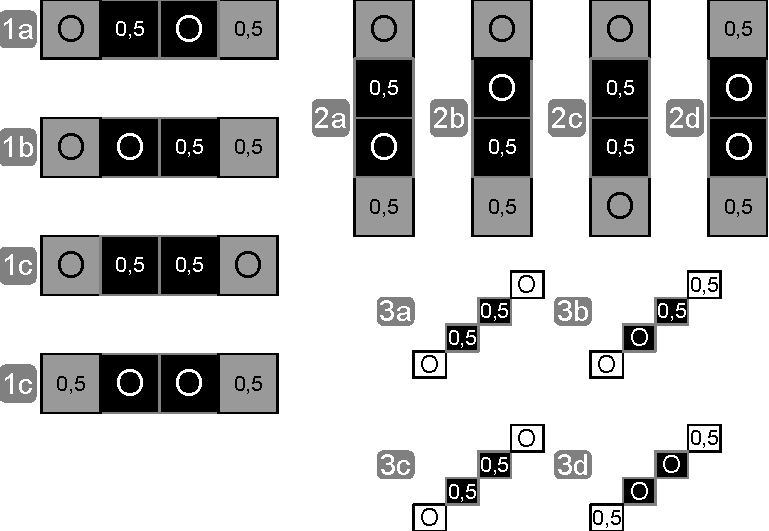
\includegraphics[scale = 0.8]{inhalt/abbildungen/verteidigung_ist_angriff.pdf}
  \caption{TicTacToe Angriffsstrategien (aus der Sicht von Bob) und Verteidigungsstrategien (aus der Sicht von Alice).}
  \label{fig:verteidigung_ist_angriff}
\end{figure}

\myparagraph{Strategieverbesserung (Value-Iteration-Algorithm)}

\subsection{Lernen ohne Strategie}
\label{subsec:Lernen ohne Strategie}

\subsection{Benutzerschnittstellen}

Alice kann ihre Kreuze auf das Spielfeld setzen, indem sie ein, vorher vom Spiel definiertes, Zahlentupel über die Tastatur eingibt. Welche Zahlentupel ein Kreuz an welche Stelle setzt ist in Abbildung \ref{fig:kreiseUndKreuzeSetzen} definiert. Sollte Alice keines der erlaubten Zahlentupel eingeben, dann wird sie darauf hingewiesen, welche Steuerungsmöglichkeiten ihr, zum setzen der Spielfiguren, zur Verfügung stehen.

\begin{figure}[!htbp]
  \centering
  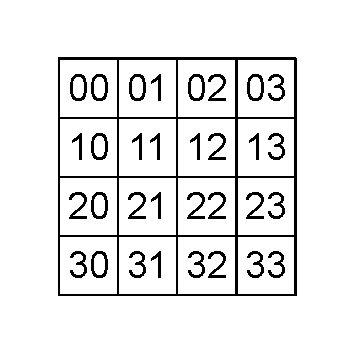
\includegraphics[scale = 1]{inhalt/abbildungen/vier_mal_vier_matrix.pdf}
  \caption{Tic Tac Toe Spielfiguren setzen}
  \label{fig:kreiseUndKreuzeSetzen}
\end{figure}

\section{Reversi}
\myparagraph{Spielprinzipien}
\myparagraph{Spielregeln}
\myparagraph{Benutzerschnittstellen}

\section{Lernverfahren}
\label{sec:lernverfahren}
\subsection{Analyse und Auswahl der lernfähigen Algorithmen}

\subsection{Anwendung der Algorithmen auf Computerspiele}

\subsection{Konzeptuelles Training der Algorithmen}

\subsection{Persistenz der Trainingsdaten}